\documentclass[11pt]{article}

\usepackage{amsmath}
\usepackage{amssymb}
\usepackage{array}
\usepackage{geometry}
\usepackage{enumitem}
\usepackage{float}
\usepackage{cancel}
\usepackage{graphicx}
\usepackage[labelformat=empty]{caption}
\usepackage{booktabs}

\geometry{
	a4paper,
 	left=20mm,
 	top=20mm,
 	bottom=20mm,
}

\setlength{\parindent}{0pt}

\newcommand{\E}{\text{E}}
\newcommand{\Var}{\text{Var}}
\newcommand{\Cov}{\text{Cov}}
\newcommand{\MSE}{\text{MSE}}

\begin{document}

\section{Wahrscheinlichkeiten}

\begin{table}[H]
\centering
\begin{tabular}{|p{2cm}|p{6cm}|p{6cm}|}
\hline
                   & \textbf{with repetition} & \textbf{without repetition} \\\hline
\textbf{ordered}   & $n^k$                         							 	  & $\frac{n!}{(n-k)!}$    \\\cline{2-3}
				   & A passcode of length $n$ with $k$ different digits           & How many ways can $k$ places be awarded to $n$ people                       \\\hline
\textbf{unordered} & $\bigl(\begin{smallmatrix}n+k-1\\k \end{smallmatrix} \bigr)$ & $\bigl(\begin{smallmatrix}n\\k \end{smallmatrix} \bigr) = \frac{n!}{k!(n-k)!}$ \\\cline{2-3}
				   & Distribute $k$ bananas (identical) to $n$ monkeys (identical)   & Select $k$ from $n$ objects                             \\\hline
\end{tabular}
\end{table}

\begin{description}[labelindent=16pt,style=multiline,leftmargin=9cm, noitemsep]
	\item[Ereignisraum $\Omega$:] Die Menge aller m{\"o}glichen Ergebnisse
	\item[Elementarereignis $\omega \in \Omega$:] Elemente vom Ereignisraum
	\item[Potenzmenge $\mathcal{P}(\Omega)$ oder $2^\Omega$:] Menge aller Teilmengen von $\Omega$
	\item[prinzipielles Ereigniss $A \subseteq \Omega$:] Kollektion von Elementarereignissen
	\item[Klasse der beobachtbaren Ereignisse $\mathcal{F}$:] Teilmenge der Potzenmenge $\mathcal{P}(\Omega)$ (alle m{\"o}glichen Ereignisse)
	\item[Wahrscheinlichkeitsmass $P: \mathcal{F} \mapsto \lbrack 0,1 \rbrack $:] Weist einem Ereignis eine Wahrscheinlichkeit zu
\end{description}

Es gelten:
\begin{equation*}
\begin{split}
	P[A^c] & = 1 - P[A] \\
	P[A \cup B] & = P[A] + P[B] - P[A \cap B] \quad\text{(Additionsregel)} \\
	P[A \cap B] & = P[B|A] \cdot P[A] \quad\text{(Multiplikationsregel)} \\
	P[A \backslash B] & = P[A] - P[A \cap B] \\
	P[A \cap B \cap C] + P[A \cap B \cap C^c] & = P[A \cap B]
\end{split}
\end{equation*}

\subsection{Diskrete Wahrscheinlichkeitsr{\"a}ume}

Ist $\Omega = {\omega_1, \omega_2,...,\omega_N}$ endlich mit $|\Omega| = N$ und $\mathcal{F} = 2^\Omega$ und sind die Elementarereignisse alle gleich wahrscheinlich, so ist $\Omega$ ein \textbf{Laplace-Raum} und $P$ die \textbf{diskrete Gleichverteilung} auf $\Omega$.

\begin{equation*}
	P[A] = \frac{\text{Anzahl der Elementarereignisse in A}}{\text{Anzahl der Elementarereignisse in $\Omega$}} = \frac{|A|}{|\Omega|}
\end{equation*}

\subsection{Bedingte Wahrscheinlichkeiten}

Die bedingte Wahrscheinlichkeit von $B$ unter der Bedingung, dass $A$ eintritt ($A$ gegeben) ist definiert durch:
\begin{equation*}
\begin{split}
	P[B|A] & := \frac{P[B \cap A]}{P[A]} \\
	P[B^c|A] & = 1-P[B|A] \\
\end{split}
\end{equation*}

\emph{Veranschaulichung:} $A$ ist eingetreten. Da $A$ und $B$ von einander abh{\"a}ngen, l{\"a}sst sich somit auch die Wahrscheinlichkeit berechnen, dass $B$ eingetreten ist.

\paragraph{Satz der totalen Wahrscheinlichkeit:} Sei $A_1,...,A_n$ eine Zerlegung von $\Omega$ in paarweise disjunkte Ereignisse, dann gilt f{\"u}r ein beliebiges Ereignis $B$:
\begin{equation*}
	P[B] = \sum_{i=1}^n P[B|A_i] P[A_i]
\end{equation*}
\begin{center}
	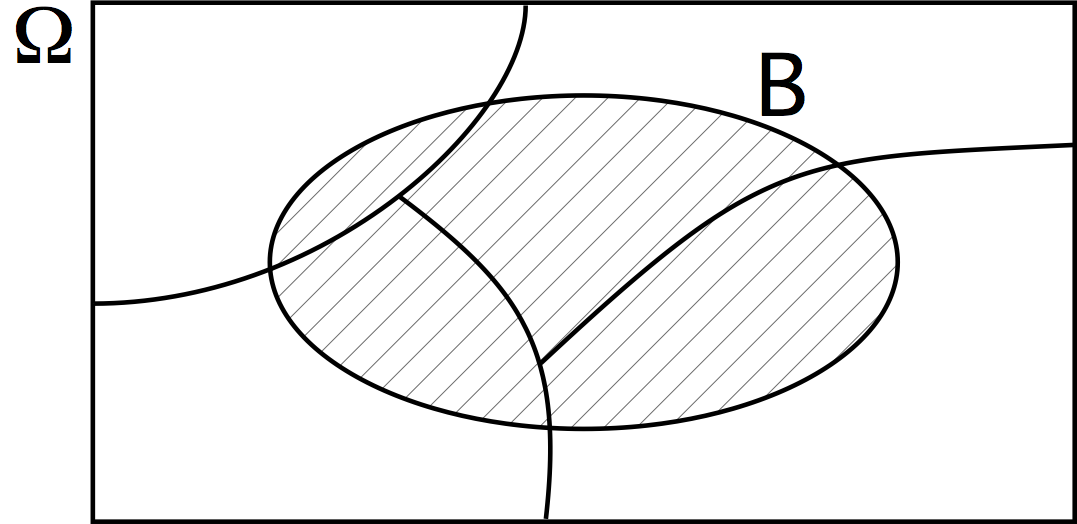
\includegraphics[width=200pt]{images/totale_wahrscheinlichkeit}
\end{center}

\paragraph{Formel von Bayes:} Ist $A_1,...,A_n$ eine Zerlegung von $\Omega$ mit $P[A_i] > 0$ und $B$ ein Ereignis mit $P[B] > 0$ so gilt f{\"u}r jedes $k$:
\begin{equation*}
	P[A_k|B] = \frac{P[B|A_k]P[A_k]}{\sum_{i=1}^n P[B|A_i]P[A_i]} = \frac{P[B|A_k]P[A_k]}{P[B]}
\end{equation*}

\subsection{Unabh{\"a}ngigkeit}

Zwei Ereignisse $A, B$ sind unabh{\"a}ngig (stochastisch), falls gilt:
\begin{equation*}
\begin{split}
	P[A \cap B] & = P[A]P[B] \quad\text{(Produktregel)}\\
	P[B|A] & = P[B] \\
	P[A|B] & = P[A] \\
\end{split}
\end{equation*}

\emph{Veranschaulichung:} Die Tatsache, dass eines der Ereignisse eingetreten ist, hat keinen Einfluss auf die Wahrscheinlichkeit des anderen. Unabh{\"a}ngigkeit und disjunkte Mengen sind jedoch \emph{nicht} das selbe.

\section{Diskrete Zufallsvariablen und Verteilungen}

\begin{description}[labelindent=16pt,style=multiline,leftmargin=8cm, noitemsep]
	\item[Zufallsvariable $X: \Omega \mapsto \mathbb{R}$:] Eine eindeutige Zuordnung, die jedem Elementarereignisses im Ereignisraum eine Zahl zuordnet.
	\item[Verteilungsfunktion $F_X: \mathbb{R} \mapsto \lbrack 0,1 \rbrack$:] $F_X(t) := P[X \leq t] := P[\{\omega | X(\omega) \leq t\}]$ \\ Der Wert an der Stelle $x$  entspricht der Wahrscheinlichkeit, dass die zugeh{\"o}rige Zufallsvarible $X$ einen Wert kleiner oder gleich $x$ annimmt.
	\item[Gewichtsfunktion $p_X:\mathcal{W}(X) \mapsto \lbrack 0,1 \rbrack$:] $p_X(x_k) := P[X = x_k] = P[\{\omega | X(\omega) = x_k\}]$ \\ Die Summe aller Gewicht aller Ereignisse muss zusammen 1 ergeben.
	\item[Verteilung $\mu_X(B)$:] $\mu_X(B) = P[X \in B] = \sum_{x_k \in B} p_X(x_k)$
	\item[Indikatorfunktion $I_A$:] $I_A(\omega) = 1$, falls $\omega \in A$, $0$ sonst. Eine diskrete Zufallsvariable, falls $\Omega$ endlich und abz{\"a}hlbar ist.
\end{description}

\subsection{Erwartungswert}

Sei $X$ eine diskrete Zufallsvariable mit Gewichtsfuntkion $p_X(x)$, dann ist der Erwartungswert $E[X]$ wie folgt definiert:
\begin{equation*}
	E[X] := \sum_{x_k \in \mathcal{W}(X)} x_kp_X(x_k) = \sum_{x_k \in \mathcal{W}(X)} x_k \cdot P[X = x_k]
\end{equation*}

Ist diese Reihe nicht \emph{absolut konvergent}, so existiert der Erwartungswert nicht.

Sei weiter $Y = g(X)$ eine Zufallsvariable gem{\"a}ss $g: \mathbb{R}\mapsto\mathbb{R}$ abh{\"a}ngig von $X$, so gilt:
\begin{equation*}
	E[Y] = E[g(X)] = \sum_{x_k \in \mathcal{W}(X)} g(x_k)p_X(x_k)
\end{equation*}

\emph{Veranschaulichung:} Der Erwartungswert beschreibt die Zahl, die der Erwartungswert im Durchschnitt annimmt.

Für Erwartungswerte gelten folgende Identitäten:
\begin{equation*}
\begin{split}
	\forall\omega: X(\omega) \leq Y(\omega) & \Rightarrow E[X] \leq E[Y] \\
	E[aX + b] & = aE[X]+b \\
	E[X^2] & = \sum_{x_k \in \mathcal{W}(X)} x_k^2 \cdot P[X = x_k] \\
	E[Z] = E[X_1 - 3X_2 + X_3] & = E[X_1] - 3E[X_2] + E[X_3]
\end{split}
\end{equation*}

Falls die Zufallsvariablen zusätzlich \textbf{unabhängig} sind:
\begin{equation*}
\begin{split}
	\E\Bigg[\prod_{i=1}^n X_i\Bigg] & = \prod_{i=1}^n E[X_i] \\
\end{split}
\end{equation*}

\subsection{Varianz}

Sei $X$ eine diskrete Zufallsvariable und ist $E[X] < \infty$, so ist die \textbf{Varianz} definiert als:
\begin{equation*}
	\Var[X] := E[(X-E[X])^2] = \sum_{x_k \in \mathcal{W}(X)}(x_k - E[X])^2 p_X(x_k)
\end{equation*}

Dementsprechend ist die \textbf{Standardabweichung} von $X$ gleich
\begin{equation*}
	\text{sd}(X) = \sigma(X) := \sqrt{\Var[X]}
\end{equation*}

Die \textbf{Kovarianz} von $X$ und $Y$ ist wie folgt definiert:
\begin{equation*}
	\Cov[X,Y] = E[XY] - E[X]E[Y] = E[(X - E[X])(Y-E[Y])]
\end{equation*}

Es gelten:
\begin{equation*}
\begin{split}
	& \Cov[X, X] = \Var[X] \\
	& \Cov[X, Y] = 0 \Rightarrow \text{$X$ und $Y$ sind unkorreliert}
\end{split}
\end{equation*}

Die Varianz wie auch die Standardabweichung beschreiben die \textbf{Streuung} der Verteilung von $X$. Je kleiner die Varianz, desto eher liegen die Werte von $X$ nahe beim Erwatungswert $E[X]$. \\

F{\"u}r beliebige Zufallsvariablen gilt:
\begin{equation*}
\begin{split}
	\Var[X] & = E[X^2] - E[X]^2 \\
	\Var[Y] & = \Var[aX +b] = a^2\Var[X] \\
	\Var\Bigg[\sum_{i=1}^n X_i \Bigg] & = \sum_{i=1}^n\Var[X_i] + 2\sum_{i<j}\Cov(X_i, X_j)
\end{split}	
\end{equation*}

Sind die Zufallsvariablen \textbf{unabhängig}, gilt:

\begin{equation*}
\begin{split}
	\Var\Bigg[\prod_{i=1}^n X_i\Bigg] & = \prod_{i=1}^n \Var[X_i] \\
	\Var\Bigg[\sum_{i=1}^n X_i \Bigg]  & = \sum_{i=1}^n\Var[X_i]
\end{split}
\end{equation*}

\subsection{Gemeinsame Verteilungen}

\begin{equation*}
\begin{split}
	\text{Gemeinsame Gewichtsfunktion } p: \mathbb{R}^n \mapsto [0,1] \qquad & p(x_1,...,x_n) := P[X_1 = x_1,..., X_n = x_n] \\
	\text{Gemeinsame Verteilungsfunktion } F: \mathbb{R}^n \mapsto [0,1] \qquad & F(x_1,...,x_n) = P[X_1 \leq x_1,..., X_n \leq x_n] \\
	& = \sum_{y_1 \leq x_1,...,y_n \leq x_n} p(y_1,...,y_n)
\end{split}
\end{equation*}

\emph{Veranschaulichung:} F{\"u}r die Zufallsvariablen $X$ und $Y$ beschreibt die gemeinsame Verteilungsfunktion die Wahrscheinlichkeit, dass der Vektor $(X,Y)$ in ein unendliches Rechteck der Form $(-\infty, X] \times (-\infty,y]$ f{\"a}llt.

\subsubsection{Randverteilungen}

Haben $X$ und $Y$ die gemeinsame Verteilungsfunktion $F$, so ist die Verteilungsfunktion der Randverteilung von $X$ gegeben durch:
\begin{equation*}
	F_X(x) := P[X \leq x] = P[X \leq x, Y < \infty] = \lim_{y \rightarrow \infty} F(x,y)
\end{equation*}

Analog dazu ist die Gewichtsfunktion der Randverteilung von $X$ gleich:
\begin{equation*}
	p_X(x) = P[X = x] = \sum_{y_i \in \mathcal{W}(Y)} P[X=x, Y=y_i] = \sum_{y_i \in \mathcal{W}(Y)} p(x, y_i) \text{ f{\"u}r } x \in \mathcal{W}(X)
\end{equation*}

\subsubsection{Unabh{\"a}ngigkeit}

Die Zufallsvariablen $X_1,...,X_n$ heissen \textbf{unabh{\"a}ngig}, falls
\begin{equation*}
\begin{split}
		\text{entweder} \quad & F(x_1,...,x_n) = F_{X_1}(x_1) \cdot\cdot\cdot F_{X_n}(x_n)  \\
		\text{oder} \quad & p(x_1,...,x_n) = p_{X_1}(x_1) \cdot\cdot\cdot p_{X_n}(x_n)
\end{split}
\end{equation*}

\begin{equation*}
	\text{unabh{\"a}ngig} \Rightarrow \text{paarweise unabh{\"a}ngig} \Rightarrow \text{unkorreliert}
\end{equation*}

\subsubsection{Korrelation}
\begin{equation*}
	\begin{split}
		\text{Corr}[X,Y]=\frac{\Cov[X,Y]}{\sqrt{\Var[X]}\sqrt{\Var[Y]}}
	\end{split}
\end{equation*}

\subsection{Bedingte Verteilungen}

Seien $X$ und $Y$ diskrete Zufallsvariablen mit gemeinsamer Gewichtsfunktion $p(x, y)$. Die bedingte Gewichtsfunktion von $X$, gegeben dass $Y = y$, ist definiert durch
\begin{equation*}
	p_{X|Y}(x|y) := P[X=x|Y=y] = \frac{P[X=x,Y=y]}{P[Y=y]} = \frac{p(x,y)}{p_Y(y)}
\end{equation*}

\section{Wichtige Diskrete Verteilungen}

\subsection{Diskrete Gleichverteilung}

Alle Elementarereignisse treten mit der gleichen Wahrscheinlichkeit auf.

\begin{equation*}
	p_X(x_k) = P[X = x_k] = \frac{1}{N}
\end{equation*}

\subsection{Bernoulli-Verteilung $X \sim Be(p) = Bin(1,p)$}

Bei einem \textbf{0-1-Experiment} ist die Gewichtsfunktion mit einer \textbf{Bernoulli-Verteilung} wie folgt definiert:
\begin{equation*}
	p_X(x) = p^x(1-p)^{1-x} \quad\text{f{\"u}r } k = 1, 2, ..., N
\end{equation*}

Es folgt, dass folgende Formeln gelten:
\begin{equation*}
\begin{split}
	p_X(1) & = P[X = 1] = p \\
	p_X(0) & = P[X = 0] = 1-p \\
\end{split}
\end{equation*}

Anders ausgedr{\"u}ckt ist $X$ die Anzahl Erfolge bei einem einzelnen 0-1-Experiment mit \textbf{Erfolgsparameter} $p$, liefert also nur die Werte 1 oder 0.

\begin{equation*}
\begin{split}
	E[X] & = p \\
	\Var[X] & = p(1-p) \quad \text{da } X^2 = X
\end{split}
\end{equation*}

\subsection{Binomialverteilung $X \sim Bin(n,p)$}

Die \textbf{Binomialverteilung} mit Parametern $n$ und $p$ beschreibt $n$ \textbf{0-1-Experimente} mit \textbf{Erfolgsparameter} $p$. \\
Der Wertebereich ist also $\mathcal{W} = \{0, 1, ..., n\}$.
\begin{equation*}
	p_X(k) = P[X = k] = \binom{n}{k}p^k(1-p)^{n-k} \quad\text{f{\"u}r } k = 0, 1, ..., n
\end{equation*}

\begin{equation*}
\begin{split}
	E[X] & = np \\
	\Var[X] & = np(1-p)
\end{split}
\end{equation*}

\subsection{Geometrische Verteilung $X \sim Geom(p)$}

Betrachten wir eine unendliche Folge von unabh{\"a}ngigen \textbf{0-1-Experimenten} mit \textbf{Erfolgsparameter} $p$, dann ist $X$ der Index der ersten Eins in der zuf{\"a}lligen 0-1-Folge. \\
Der Wertebereich ist dementsprechend $\mathcal{W} = \mathbb{N}$.
\begin{equation*}
	p_X(k) = P[X = k] = p(1-p)^{k-1} \quad\text{f{\"u}r } k = 1, 2, 3,...
\end{equation*}

$X = k$ heisst gerade, dass $A_1,..., A_{k-1}$ nicht eintreten und $A_k$ als erstes eintritt.
\begin{equation*}
\begin{split}
	E[X] & = \frac{1}{p} \\
	\Var[X] & = \frac{1-p}{p^2}
\end{split}
\end{equation*}

\emph{Bermerkung:} Hat das "forgetfulness property"

\subsection{Negativbinomiale Verteilung $X \sim NB(r,p)$}

Eine \textbf{negativbinomiale Verteilung} mit Parametern $r$ und $p$ beschreibt eine unendliche Folge von unabh{\"a}ngigen \textbf{0-1-Experimenten} mit \textbf{Erfolgsparameter} $p$ und dem $r$-ten Erfolg. \\
Der Wertebereich ist $\mathcal{W} = \{r, r+1, r+2,...\}$.
\begin{equation*}
	p_X(k) = P[X = k] = \binom{k-1}{r-1}p^r(1-p)^{k-r} \quad\text{f{\"u}r } k = r, r+1, r+2, ...
\end{equation*}

\begin{equation*}
\begin{split}
	E[X] & = \frac{r}{p} \\
	\Var[X] & = \frac{r(1-p)}{p^2}
\end{split}
\end{equation*}

\subsection{Hypergeometrische Verteilung}

In einer Urne seien $n$ Gegenst{\"a}nde, davon $r$ vom Typ 1 und $n -r$ vom Typ 2. Man zieht ohne Zur{\"u}cklegen $m$ der Gegenst{\"a}nde; die Zufallsvariable $X$ beschreibe die Anzahl der Gegenst{\"a}nde vom Typ 1 in dieser Stichprobe vom Umfang $m$. Dann hat $X$ eine \textbf{hypergeometrische Verteilung} mit Parametern $n \in \mathbb{N}$ und $m,r \in \{1, 2, ..., n\}$. \\
Der Wertebereich ist gleich $\mathcal{W} = \{1, 2,... \min(r, m)\}$.
\begin{equation*}
	p_X(k) = \frac{\binom{r}{k}\binom{n-r}{m-k}}{\binom{n}{m}} \quad \text{f{\"u}r } k \in \mathcal{W}(X)
\end{equation*}

\subsection{Poisson-Verteilung $X \sim \mathcal{P}(\lambda)$}

Die \textbf{Poisson-Verteilung} mit Parameter $\lambda \in (0, \infty)$ beschreibt die Anzahl Ereignisse in einem Zeitintervall. Sie ist eine Verteilung auf der Menge $\mathbb{N}_0$.
\begin{equation*}
	p_X(k) = e^{-\lambda}\frac{\lambda^k}{k!}\quad\text{f{\"u}r } k = 0, 1, 2,...
\end{equation*}

\begin{equation*}
\begin{split}
	E[X] & = \lambda \\
	\Var[X] & = \lambda
\end{split}
\end{equation*}

\section{Allgemeine Zufallsvariablen}

Das \textbf{stochastiche Verhalten} einer \textbf{allgemeinen Zufallsvariable} $X$ wird durch ihre Verteilung beschrieben:
\begin{equation*}
	\mu_X(B) := P[X \in B] 
\end{equation*}

Die \textbf{Verteilungsfunktion $F_X$} ist durch $\mu_X$ festgelegt:
\begin{equation*}
	F_X(t) = P[X \leq t] = \mu_X(]-\infty,t])
\end{equation*}

Die \textbf{Dichtefunktion} $f_X: \mathbb{R} \mapsto [0,\infty[$ ist das allgemeine Analog zur Gewichtsfunktion. Die Zufallsvariable wird \textbf{(absolut) stetig}, falls gilt:
\begin{equation*}
	F_X(t) = \int_{-\infty}^t f_X(s)\ ds \quad\text{f{\"u}r alle }t\in \mathbb{R}
\end{equation*}

Die Dichtefunktion $f_X$ hat folgende Eigenschaften:
\begin{equation*}
\begin{split}
	f_X \geq 0 \text{ und } f_X & = 0\text{ ausserhalb von } \mathcal{W}(X) \\
	\int_{-\infty}^\infty f_X(s)\ ds & = 1
\end{split}
\end{equation*}

\begin{equation*}
	\textbf{Dichtefunktion} = \textbf{Ableitung der Verteilungsfunktion}
\end{equation*}

\subsection{Erwartungswerte}

Ist $X$ stetig mit Dichte $f_X(x)$, so ist der Erwartungswert gleich
\begin{equation*}
	E[X] = \int_{-\infty}^\infty x f_X(x)\ dx
\end{equation*}
sofer das Integral absolut konvergiert.

Sei weiter $X$ und $Y = g(X)$ zwei Zufallsvariablen. Ist $X$ stetig mit Dichte $f_X(x)$, so ist
\begin{equation*}
	E[Y] = E[g(X)] = \int_{-\infty}^\infty g(x)f_X(x)\ dx
\end{equation*} 

\subsection{Gemeinsame Verteilungen, unabh{\"a}ngige Zufallsvariablen}

Die \textbf{gemeinsame Verteilungsfunktion} von $n$ Zufallsvariablen $X_1,...,X_n$ ist die Abbildung $F: \mathbb{R}^n \mapsto [0,1]$
\begin{equation*}
	F(x_1,...,x_n) = \int_{-\infty}^{x_1} ... \int_{-\infty}^{x_n} f(t_1,...,t_n)\ dt_n...dt_1
\end{equation*}

Somit ist $f: \mathbb{R}^n \mapsto [0, \infty[$ die \textbf{gemeinsame Dichte} von $X_1,...,X_n$.

\subsection{Transformationen}

Sei $X$ eine Zufallsvariable mit Verteilungsfunktion $F_X$ und Dichte $f_X$. Betrachten wir nun die Transformation $g: \mathbb{R} \mapsto \mathbb{R}$ und die neue Zufallsvariable $Y = g(X)$. Wie sieht nun $F_Y$ und $f_Y$ aus?

\begin{equation*}
	\textbf{Ansatz:}\quad F_Y(t) = P[Y \leq t] = P[g(X) \leq t] = \int_{A_g} f_X(s)\ ds
\end{equation*}

\subsubsection{Affin/Linear: $g(x) = ax + b$}

\begin{equation*}
\begin{split}
	F_Y(t) & = F_X(\frac{t-b}{a}) \\
	f_Y(t) & = \frac{d}{dt} F_Y(t) = \frac{1}{a}f_X(\frac{t-b}{a})
\end{split}
\end{equation*}

\subsubsection{Nichtlinear: $g(x) = x^2$}

\begin{equation*}
\begin{split}
	F_Y(t) & = F_X(\sqrt{t}) - F_X(-\sqrt{t}) \\
	f_Y(t) & = \frac{1}{\sqrt{2\pi}}t^{-\frac{1}{2}}e^{-\frac{1}{2}t} \quad\text{für}\quad t \geq 0
\end{split}
\end{equation*}

\subsubsection{Nichtlinear: $g(x) = \frac{1}{x}$}

\begin{equation*}
\begin{split}
	F_Y(t) & = 1 - F_X(\frac{1}{t}) \\
	f_Y(t) & = \frac{1}{t^2}f_X(\frac{1}{t})
\end{split}
\end{equation*}

\subsection{Randverteilungen}

Haben $X$ und $Y$ die gemeinsame Verteilungsfunktion $F$, so ist die \textbf{Verteilungsfunktion der Randverteilung} von $X$ gleich
\begin{equation*}
	F_X(x) := P[X \leq x] = P[X \leq x, Y < \infty] = \lim_{y \rightarrow\infty}F(x,y)
\end{equation*}

Sei weiter $f(x,y)$ die gemeinsame Dichte, so ist analog zur Gewichtsfunktion $p_X$  die \textbf{Dichtefunktion der Randverteilung} von $X$ gleich
\begin{equation*}
	f_X(x) = \int_{-\infty}^\infty f(x,y) dy
\end{equation*}

\section{Wichtige stetige Verteilungen}

\subsection{Gleichverteilung $X \sim \mathcal{U}(a,b)$}

Die \textbf{Gleichverteilung} auf einem Intervall $[a,b]$ ist ein Modell f{\"u}r die zuf{\"a}llige Wahl eines Punktes in $[a,b]$. Die Zufallsvariable $X$ hat somit den Wertebereich $\mathcal{W} = [a,b]$.
\begin{equation*}
\begin{split}
	f_X(t) = \begin{cases}
		\frac{1}{b-a}\quad\text{f{\"u}r }a\leq t \leq b \\
		0\quad\text{sonst }
	\end{cases} \\
	F_X(t) = \begin{cases}
		0\quad\text{f{\"u}r } t < a \\
		\frac{t-a}{b-a}\quad\text{f{\"u}r } a \leq t \leq b \\
		1\quad\text{f{\"u}r } t > b
	\end{cases}
\end{split}
\end{equation*}

\begin{equation*}
\begin{split}
	E[X] & = \frac{a+b}{2} \\
	\Var[X] & = \frac{1}{12}(b-a)^2
\end{split}
\end{equation*}

\subsection{Exponentialverteilung $X \sim Exp(\lambda) = Ga(1, \lambda)$}

Die \textbf{Exponentialverteilung} mit Parameter $\lambda > 0$ ist das stetige Analog der \textbf{geometrischen Verteilung}. \\
Die Zufallsvariable $X$ hat $\mathcal{W} = [0, \infty[$.
\begin{equation*}
\begin{split}
	f_X(t) & = \begin{cases}
		\lambda e^{-\lambda t}\quad\text{f{\"u}r } t \geq 0 \\
		0 \quad\text{f{\"u}r } t < 0 \\
	\end{cases} \\
	F_X(t) & = \int_{-\infty}^t f_X(s)\ ds = \begin{cases}
		1 - e^{-\lambda t} \quad\text{f{\"u}r } t \geq 0 \\
		0 \quad\text{f{\"u}r } t < 0 \\
	\end{cases}
\end{split}
\end{equation*}

Wie die geometrische Verteilung ist die Exponentialverteilung ein Modell f{\"u}r Wartezeiten oder Lebensdauern (forgetfulness property). \\
Die Summe $n$ unabhängiger, $Exp(\lambda)$-verteilter Zufallsvariablen ist $Ga(n, \lambda)$-verteilt.

\subsubsection{Gamma-Verteilung $Z \sim Ga(\alpha, \lambda)$}

\begin{equation*}
	f_Z(z) = \frac{1}{\Gamma (\alpha)}\lambda^\alpha z^{\alpha-1} e^{-\lambda z} \quad\text{mit}\quad \Gamma(\alpha) := \int_0^\infty u^{\alpha-1}e^{-u}\ du
\end{equation*}
\begin{equation*}
	\text{wobei}\quad \Gamma(n) = (n-1)! \quad \forall \alpha = n \in \mathbb{N}
\end{equation*}

\subsection{Normalverteilung $X \sim \mathcal{N}(\mu, \sigma^2)$}

Die \textbf{Normalverteilung} (NV, auch \textbf{Gauss-Verteilung}) hat zwei Parameter, $\mu \in \mathbb{R}$ und $\sigma^2 > 0$. Der Wertebereich entspricht $\mathcal{W} = \mathbb{R}$.
\begin{equation*}
	f_X(t) = \frac{1}{\sigma\sqrt{2\pi}}e^{-\frac{(t-\mu)^2}{2\sigma^2}}\quad\text{f{\"u}r } t \in \mathbb{R}
\end{equation*}

\begin{equation*}
\begin{split}
	E[X] & = \mu \\
	\Var[X] & = \sigma^2 \\
\end{split}
\end{equation*}

\subsubsection{Standard-Normalverteilung $X \sim \mathcal{N}(0, 1)$}

Weder die Dichte $\varphi(t)$ noch die Verteilungsfunktion $\Phi(t)$ k{\"o}nnen mit einer geschlossenen Formel ausgedr{\"u}ckt werden, das Integral ist jedoch \textbf{tabelliert}:
\begin{equation*}
	\Phi(t) = \int_{-\infty}^t \varphi(s)\ ds = \frac{1}{\sqrt{2\pi}}\int_{-\infty}^t e^{-\frac{1}{2}s^2}\ ds
\end{equation*}

\begin{equation*}
	F_X(t) = P[X \leq t] = \Phi(\frac{t-\mu}{\sigma})
\end{equation*}

\subsection{Cauchy-Verteilung}

Eine \textbf{Cauchy-verteilte} Zufallsvariable $X$ hat den Wertebereich $\mathcal{W} = \mathbb{R}$.
\begin{equation*}
\begin{split}
	f_X(x) & = \frac{1}{\pi}\frac{1}{1+x^2}\quad\text{f{\"u}r }x \in \mathbb{R} \\\
	F_X(x) & = \frac{1}{2}+\frac{1}{\pi}\arctan(x)\quad\text{f{\"u}r }x \in \mathbb{R}
\end{split}
\end{equation*}

Die Cauchy-Verteilung ist eine \textbf{langschw{\"a}nzige Verteilung}, dies, weil $X$ auch noch sehr grosse Werte mit substantieller Wahrscheinlichkeit annimmt.

\begin{equation*}
	E[X] = \text{undefiniert}
\end{equation*}

\section{Ungleichungen und Grenzwerte}

\subsection{Ungleichungen}

\subsubsection{Markov-Ungleichung}

Sei $X$ eine Zufallsvariable und ferner $g: \mathcal{W}(X) \mapsto [0, \infty[$ eine wachsende Funktion. F{\"u}r jedes $c \in mathbb{R}$ gilt dann
\begin{equation*}
	P[X \geq c] \leq \frac{E[g(X)]}{g(c)}
\end{equation*}

\subsubsection{Chebyshev-Ungleichung}

Sei $Y$ eine Zufallsvariable mit endlicher Varianz. F{\"u}r jedes $b > 0$ gilt dann
\begin{equation*}
	P[|Y - E[Y]| \geq b] \leq \frac{\Var[Y]}{b^2}
\end{equation*}

\subsection{Gesetz der grossen Zahlen (GGZ)}

Sei $X_1, X_2, ...$ eine Folge von unabh{\"a}ngigen Zufallsvariablen (i.i.d.) mit dem Erwartungswert $E[X_i] = \mu$ und der Varianz $\Var[X_i] = \sigma^2$. Sei $\overline{X}_n = \frac{1}{n}S_n = \frac{1}{n}\sum_{i=1}^n X_i$. Dann \textbf{konvergiert} $\overline{X}_n$ f{\"u}r $n \mapsto \infty$ in Wahrscheinlichkeit gegen $\mu = E[X_i]$:
\begin{equation*}
\begin{split}
	\text{schwach:} & \qquad P[|\overline{X}_n - \mu| > \varepsilon] \xrightarrow{n \mapsto \infty} 0 \\
	\text{stark:} & \qquad \overline{X}_n \xrightarrow{n\mapsto\infty}\mu,\ P[\{\omega \in \Omega\ |\  \overline{X}_n(\omega) \xrightarrow{n\mapsto\infty}\mu\}] = 1 
\end{split}
\end{equation*}

Das heisst, dass mit beliebig grosser Wahrscheinlichkeit $1- \delta$ der Wert von $\overline{X}_n$ f{\"u}r hinreichend grosse $n$ beliebig nahe (bis auf $\varepsilon$) bei $\mu$ liegt.

\subsection{Zentraler Grenzwertsatz (ZGS)}

Sei $X_1, X_2, ...$ eine Folge von i.i.d. Zufallsvariablen mit $E[X_i] = \mu$ und $\Var[X_i] = \sigma^2$. F{\"u}r die Summe $S_n = \sum_{i=1}^n X_i$ gilt dann
\begin{equation*}
	\lim_{n\rightarrow\infty} P[\frac{S_n - E[S_n]}{\sqrt{\Var[S_n]}} \leq x] =	\lim_{n\rightarrow\infty} P[\frac{S_n - n\mu}{\sigma \sqrt{n}} \leq x] = \Phi(x)
\end{equation*}
wobei $\Phi$ die Verteilungsfunktion der $\mathcal{N}(0,1)$-Verteilung ist.

\subsection{Grosse Abweichungen und Chernoff-Schnranken}

Die \textbf{momenterzeugende Funktion} einer Zufallsvariable $X$ ist
\begin{equation*}
	M_X(t) := E[e^{tX}]
\end{equation*}
Sie ist immer wohldefiniert in $[0, \infty[$.

Seien $X_1, ..., X_n$ i.i.d. Zufallsvariablen, f{\"u}r welche die momenterzeugende Funktion $M_X(t)$ f{\"u}r alle $t \in \mathbb{R}$ endlich ist. F{\"u}r jedes $b \in \mathbb{R}$ gilt dann:
\begin{equation*}
	P[S_n > b] \leq \exp(\inf_{t \in \mathbb{R}}(n \log M_X(t) - tb))
\end{equation*}

\section{Sch{\"a}tzer}

\begin{description}[labelindent=16pt,style=multiline,leftmargin=6cm, noitemsep]
	\item[Sch{\"a}tzer $T$:] Eine Zufallsvariable
	\item[Sch{\"a}tzwert:] Ist eine Zahl $T_j(\omega) = t_j(x_1,...,x_n)$, also das Ergebnis einer konkreten Berechnung
	\item[erwartungstreuer Sch{\"a}tzer:] Falls $\E_\vartheta[T] = \vartheta$, $T$ sch{\"a}tzt im Durchschnitt also richtig
	\item[Bias/Sch{\"a}tzfehler:] $\E_\vartheta[T] - \vartheta$ (0 falls $T$ erwartungstreu ist)
	\item[MSE:] Mittlerer quadratische Sch{\"a}tzfehler\\ $\MSE_\vartheta[T] := \E_\vartheta[(T-\vartheta)^2]$
	\item[konsistent:] Eine Folge von Sch{\"a}tzern $T^{(n)},\ n\in\mathbb{N}$, falls \\ $\lim_{n \rightarrow \infty} P_\vartheta[|T^{(n)} -\vartheta| > \varepsilon] = 0$
\end{description}

\emph{Bemerkung:} F{\"u}r erwartungstreue Sch{\"a}tzer sind die Varianz und MSE dasselbe:
\begin{equation*}
	\MSE_\vartheta[T] = \E_\vartheta[(T-\vartheta)^2] = \Var_\vartheta[T] + (\E_\vartheta[T] - \vartheta)^2
\end{equation*}

\subsection{Maximum-Likelihood-Methode (ML-Methode)}

Seien in einem Modell $P_\vartheta$ die Zufallsvariablen $X_1,...,X_n$ entweder diskret mit der geimensamen Gewichtsfunktion $p(x_1,...,x_n;\vartheta)$ oder stetig mit $f(x_1,...,x_n;\vartheta)$. Die \textbf{Likelihood-Funktion} ist dann definiert als:
\begin{equation*}
	L(x_1,...,x_n;\vartheta) := \begin{cases}
		p(x_1,...,x_n; \vartheta), \text{im diskreten Fall} \\
		f(x_1,...,x_n; \vartheta), \text{im stetigen Fall}
	\end{cases}
\end{equation*}

\section{Tests}

Das Grundproblem ist, eine Entscheidung zwischen zwei konkurrierenden Modellklassen zu treffen, der \textbf{Hypothese $\Theta_0 \subseteq \Theta$} und der \textbf{Alternative $\Theta_A \subseteq \Theta$}, wobei $\Theta_0 \cap \Theta_A = \emptyset$.

\begin{center}
	Hypothese $H_0$: $\vartheta \in \Theta_0$ \\
	Alternative $H_A$: $\vartheta \in \Theta_A$
\end{center}

Die Hypothese $H_0$ besagt also, dass der wahre (aber unbekannte) Parameter $\vartheta$ in der Menge $\Theta_0$ liegt. \\
Hypothesen und Alternativen heissen \textbf{einfach}, falls sie nur aus einem einzelnen Wert besteht, sonst heissen sie \textbf{zusammengesetzt}. \\

Ein \textbf{Test} ist nun allgemein eine Entscheidungsregel, die zu gegebenen Daten $x_1,...,x_n$ einen von zwei Werten liefert; dabei nimmt man als diese zwei Werte 0 und 1, und man interpretiert den Wert 1 als die Entscheidung, die Hypothese $H_0$ bzw. $\Theta_0$ abzulehnen. Konkreter ausgedr{\"u}ckt bestimmt man einen \textbf{Verwerfungsbereich} $K \subseteq \mathbb{R}$. Man verwirft dann die Hypothese, wenn der realisierte Wert in den Verwerfungsbereich $K$ f{\"a}llt. \\

Es werden folgende Fehler unterscheidet:
\begin{description}[labelindent=16pt,style=multiline,leftmargin=4cm, noitemsep]
	\item[Fehler 1. Art:] Die Hypothese wird zu Unrecht abgelehnt, obwohl sie richtig ist
	\item[Fehler 2. Art:] Die Hypothese wird zu Unrecht nicht verworfen. Man akzeptiert also die Hypothese, obwohl sie falsch ist.
\end{description}


\end{document}
